%
% This is Chapter 5 file (chap5.tex)
%
\chapter{Contextual Suggestion}
The increasing use of mobile devices enables an information retrieval (IR) 
system to capitalize on various types of contexts 
(e.g., temporal and geographical information) about its users. 
Combined with the user preference history recorded in the system, 
a better understanding of users' information need can be achieved and 
it thus leads to improved user satisfaction. More importantly, such a 
system could {\em proactively} recommend suggestions based on the contexts.

User profiling is essential and is the key to success in contextual suggestion. 
Since user's preference is always modeled as long-term and static we include 
it as part of the context of this problem.
Given most users' observed behaviors are sparse and their preferences are 
latent in an IR system, constructing accurate user profiles is generally 
difficult. In our work, we focus on location-based contextual suggestion 
and propose two approaches to construct user profiles. 

The first approach uses the categories and/or descriptions from 
users' activities history to build user profile. The rationale here is 
that users are at a better chance to favor the places that are similar 
to what she liked before in terms of the category/description of the places. 
In reality, one user would typically have several positively rated and also 
several negatively rated suggestions in the past. We compute the similarity 
of category/description between each candidate suggestion and all 
places in the user's activity history and combine the averages of 
both positive and negative scores. 

The second approach leverages the users' opinions to form the user profiles. 
By assuming users would like or dislike a place with similar reasons, 
we construct the opinion-based user profile in a collaborative way: 
opinions from the other users are leveraged to estimate a profile for 
the target user. Candidate suggestions are represented in the same fashion 
and ranked based on their similarities with respect to the user profiles.

Moreover, we also develop a novel summary generation method that utilizes 
the opinion-based user profiles to generate personalized and high-quality 
summaries for the suggestions. 

Experiments conducted over three standard TREC Contextual suggestion 
collections and a Yelp data set show the advantage of our approaches and 
the system developed based on the proposed methods have been ranked as 
top 1 in both TREC 2013 and 2014 Contextual Suggestion tracks.

% \section{Introduction}

% The increasing availability of internet access on
% mobile devices, such as smart phones and tablets,
% has made mobile search a new focus of information retrieval (IR) research community.
% The contextual information such as geographical and temporal 
% information that is available in mobile search environment provides 
% unique opportunities for IR systems 
% to better understand its users. Moreover, a user's preference history 
% collected in a mobile search system can be incorporated with such 
% contextual information to better understand the user's informational need. 
% Ideally, a mobile search system should thus {\em proactively} generate 
% suggestions for various user information needs.  
% For example, it would be useful to automatically send recommendations about 
% the Beatles museum to a music fan who travels to Liverpool. In addition to 
% returning a list of suggestions to the user, it would also be useful 
% to provide a short yet \textit{informative summary} for each suggestion so that 
% the user can easily decide whether the recommended suggestion is interesting 
% before accepting it. This problem is referred to as {\em contextual suggestion}, 
% and has been identified as one of the IR challenges (i.e,. ``finding what you 
% need with zero query terms'') in the SWIRL 2012 workshop \cite{allan:2012}.


\section{Problem Formulation} 
\label{sec:chap5prob}

The problem of contextual suggestion can be formalized 
as follows. Given a user's contexts (e.g., location
and time) and the her/his preferences on a few example
suggestions, the goal is to retrieve candidate 
suggestions that can satisfy the user's information 
need based on both the context and preferences. 
For each returned candidate suggestion, a short description 
may also be returned so that the user could decide whether 
the suggestion is interesting without going to its website.
For example, assume that a user liked ``Magic Kingdom Park'' 
and ``Animal Kingdom'', but disliked ``Kennedy Space Center''. 
If the user is visiting Philadelphia on a Saturday, the system 
is expected to return a list of suggestions such as ``Sesame Palace'' 
together with a short summary of each suggestion, 
e.g., ``Sesame Place is a theme park in Langhorne, Pennsylvania based on 
the Sesame Street television program. It includes a variety of rides, shows, 
and water attractions suited to very young children.''

Since our paper focuses on user modeling, we assume 
that we have filtered out the suggestions that do not meet the context requirement 
and the remaining suggestions
only need to be ranked based on the relevance to 
user preferences. Note that the filtering process 
based on contexts can be achieved by simply removing 
the suggestions that do not satisfy the contextual 
requirements, such as the ones that are either 
too far away from the current location or those 
that are currently closed. 

The remaining problem is essentially a ranking 
problem, where candidate suggestions need to 
be ranked based on how relevant the suggestions
are with respect to a user's interest. 
Formally, let $U$ denote a user and $CS$ denote a 
candidate suggestion, we need to estimate 
$S(U,CS)$, i.e., the relevance score between 
the user and the suggestion. 

It is clear that the estimation of the relevance 
score is related to how to represent $U$ 
and $CS$ based on the available information. 
Let us first look at what kind of 
information we can gather for $U$ and $CS$.  
For each user $U$, 
we know the user's preferences (i.e., ratings) for a list of 
example suggestions. We denote an example suggestion $ES$ 
and its rating given by user $U$ as $R(U,ES)$.  For a 
suggestion (either $CS$ or $ES$), we assume that the 
following information about the suggestion is available: 
the text description such as title and category and online 
opinions about this suggestion. 
Note all the information can be collected from online location 
services such as Yelp and Tripadvisor. 


\section{Category and Description based User Profile Modeling}

\subsection{Ranking based on User Profiles}

We first describe our framework of how to rank candidate suggestions 
based on user profiles. How to use the category and description to build 
user profile will be introduced later. 
The profile of each user consists of the user's 
preferences for example suggestions. The suggestions that a 
user likes are referred to as ``positive user profile'', and those
disliked by the user are referred to as ``negative user profile''. 
Intuitively, the relevance score of a candidate suggestion should 
be higher when it is similar to positive user profile while different
from the negative user profile. 

Formally, we denote $U$ as a user and $CS$ as a candidate suggestion. 
Moreover, let ${\cal U}_{+}(U)$ denote positive user profile, 
i.e., a set of places that the user likes, 
and ${\cal U}_{-}(U)$ denote negative user profile, i.e., a set 
of places that the user dislikes. The relevance score of $CS$ with 
respect to $U$ can then be computed as follows:  
\begin{eqnarray}
    \mathrm{S(U,CS)} &=& \varphi \times \mathrm{SIM}({\cal U}_{+}(U),CS) + (1-\varphi) \times \mathrm{SIM}({\cal U}_{-}(U),CS) \\
&=& \varphi \times \frac{\sum_{e \in {\cal U}_{+}(U)}{\mathrm{SIM}(e,CS)}}{|{\cal U}_{+}(U)|} 
+ (1-\varphi) \times \frac{\sum_{e \in {\cal U}_{+}(U)}{\mathrm{SIM}(e,CS)}}{|{\cal U}_{+}(U)|} 
\label{chap5_eq1}
\end{eqnarray}
where $\varphi \in [0,1]$ regularizes the weight between the 
positive and negative similarities. When $\varphi=1$, the highly ranked 
suggestions would be those similar to the suggestions that the user likes. 
When $\varphi=0$, the highly ranked suggestions would be those 
different from the suggestions that the user dislikes. 
$\mathrm{SIM}({\cal U}_{+}(U),CS)$ measures the similarity between the 
positive user profile and the candidate suggestion, 
and we assume that it can be computed 
by averaging the similarity scores between each positive example and 
the candidate suggestion. $|{\cal U}_{+}(U)|$ corresponds to the number of 
positive examples in the user profile. It is trivial to explain the 
corresponding symbols for negative one.

Thus, it is clear that the problem of computing the relevance score 
of a candidate suggestion with respect to a user can be boiled down 
to the problem of computing the relevance score between a candidate
suggestion and a place mentioned in the user profile, i.e., $\mathrm{SIM}(e,CS)$, 
where $e$ is an example from the user profile. We explore the following 
two types of information to compute $\mathrm{SIM}(e,CS)$: (1) the category 
of a place; and (2) the description of a place. 


\subsubsection{Category-based Similarity}
Category is a very important factor that may greatly impact user preferences. 
However, the categories of the suggestions are often in hierarchical format. 
Here is an example category, 
\textit{[History Museum$\to$Museum$\to$Arts].}
The categories becomes more general from the left to the right. 
In this example, \textit{Arts} is the most general category
while \textit{History Museum} is the most specific category.
Note that we represent the hierarchical categories
as a set of categories in this paper. 


\begin{table}[t]
\begin{center}
\caption{Examples of Categories in Example Suggestions}\label{tb:category_example}
\begin{tabular}{ | l | p{6.5cm} |}
\hline
\textbf{NAME} & \textbf{Categories} \\ 
\hline
\hline
HoSu Bistro & SushiRestaurant$\to$Restaurants;
             KoreanRestaurant$\to$Restaurants;
            JapaneseRestaurant$\to$Restaurants
\\ 
\hline
The Rex & JazzBlues$\to$MusicVenues$\to$Arts 
\\ 
\hline
St. Lawrence Market & Grocery$\to$Shopping;
                    FarmersMarket$\to$Shopping 
\\ 
\hline
... & ... \\
\hline
\end{tabular}
\end{center}
\end{table}
We can compute $\mathrm{SIM}(e,CS)$ based on the category similarities between 
$e$ and $CS$ as follows: 
\begin{equation}
\mathrm{SIM}_{\cal C}(e,CS) = \frac{ \sum_{c_i \in {\cal C}(e)} \sum_{c_j \in {\cal C}(C)} \frac{|Intersection(c_i,c_j)|}{max(|c_i|,|c_j|)}}{|{\cal C}(e)| \times |{\cal C}(C)|} 
\label{chap5_eq2}
\end{equation}
where
${\cal C}(e)$ denotes the set of categories of location $e$ and
$|Intersection(c_i,c_j)|$ is the number of common categories 
between $c_i$ and $c_j$. 
Recall that we crawled the candidate suggestions from two online 
sources. Table~\ref{tb:category_example} shows some example categories 
of the suggestions.

\subsubsection{Description-based Similarity}
In example suggestions, each suggestion has its unique 
description which typically is at a short length. We want 
to learn how the descriptions can affect people's decision 
on different places. By comparing the descriptions of training 
suggestions with textual web sites of testing suggestions we 
may find some interesting connections. We use textual web sites 
of testing suggestions because we believe that textual web sites 
are more reliable than descriptions especially when we rank 
candidate suggestions. The similarity used function is 
the F2EXP ranking function \cite{Fang:2005:EAA:1076034.1076116} since it has been shown to be effective 
for long queries \cite{Fang:2005:EAA:1076034.1076116}. So, we have 
\begin{equation}
\mathrm{F2EXP}(a,b)=\sum_{t\in{a\cap b}}{\frac{c(t,b)}{c(t,b)+0.5+\frac{0.5\cdot |b|}{avdl}\cdot (\frac{N+1}{df(t))})^{0.35}}}
\label{chap5_eq3}
\end{equation}
Thus, we compute the similarity scores as follows: 
\begin{equation}
\mathrm{SIM}_{\cal D}(e,CS) = \mathrm{F2EXP}(DES(e),DES(CS))
\label{chap5_eq4}
\end{equation}
where $\mathrm{DES}(e)$ is a description of the example place $e$. 


\section{Opinion-based User Profile Modeling}  \label{sec:user} 

\subsection{Basic Idea} 

In our problem setup, the available information for a user $U$ includes 
the user's preferences for a set of example suggestions. 
Existing studies often estimated user profiles based on the descriptive 
information of the example suggestions such as their names, descriptions and 
web sites 
\cite{Yang:2013:OUP:2499178.2499191,udel:treccs2013,udel:treccs2012, 
irit:treccs2012, udben:treccs2012,uamst:treccs2013,cwi:treccs2013}. 
However, one limitation of this approach is that such descriptive information 
could be very specific for one suggestion and might not be useful at all to 
infer the user's preferences on other suggestions. Categories of the suggestions 
were then used by some methods to overcome the limitation  
\cite{georgetown:treccs2012,udel:treccs2012,isi:treccs2013}. 
Although this method improves the performance, the improvement is often 
limited since category information might be too general to capture the 
reasons behind the user preferences. 

\begin{figure}[t]
\centering
    \includegraphics[width=1.0\textwidth]{figures/irj_fig1.eps}
    \caption{An example scenario when we know the user's 
    preferences for some suggestions and want to 
    predict the preference for the unknown one}
    \label{chap5_fig0}
\end{figure}

Instead of simply capturing what a user likes or dislikes, 
i.e. the descriptive information of example suggestions, we propose to 
model the user profile based on the user's opinions about the example suggestions. 
The opinions about a suggestion is defined as the $\langle$ rating, 
review text $\rangle$ pairs in our paper.  
When determining whether an opinion is positive or negative, we rely on the 
numeric rating rather than the review text. 
More details about this are described in Section \ref{sec:design}. 

We now motivate the opinion-based user modeling through an example as shown 
in Figure \ref{chap5_fig0}. 
Assume that we know a user's preferences for the first four suggestions and 
want to infer the user preference for the last one. Neither description-based 
nor category-based methods are effective here. For example, the category of 
the candidate suggestion is ``hotel'', which does not match with the categories 
of all the example suggestions. Moreover, the descriptions of these example 
suggestions are very specific, making it difficult to find their commonalities. 
However, if we are able to know the user's preference and review for each 
example suggestion, it would be possible for us to more accurately infer why 
the user liked or disliked these places. 
For example, it seems that the two suggestions that the user liked 
(i.e., example suggestions 1 and 3) are ``clean'' while the places that the 
user disliked (i.e., example suggestions  2 and 4) are both 
``dirty''. Thus, we may infer that the user prefers places that are 
``clean''. Now if we know that a candidate suggestion is well known for 
its ``cleanness'' based on online reviews, we could safely infer 
that the user would like this candidate suggestion. Clearly, opinion-
based user profile modeling should be more effective than the category-
based and description-based methods since it can capture user 
preferences more accurately. 


One challenge of using opinions to model user profile is that users may 
not share their opinions explicitly by writing the reviews for each 
example suggestion. To address the challenge, we propose to leverage 
opinions from similar users. More specifically, we assume that users 
who rate a suggestion similarly would share the similar opinions about 
the suggestion. If a user likes a suggestion, we could identify all 
other users who also like this suggestion and leverage their reviews 
about the suggestion as part of the user's positive profile, i.e., the 
profile about what the user likes. We can build the negative profile in 
a similar way.

Specifically, we use positive reviews of the example suggestions that the 
user likes to build his or her positive user profile, and use negative
reviews of example suggestions that the user dislikes to build negative user 
profile. The basic assumption is that the opinion of a user about a place 
can be inferred by the opinions of the users who share the same preference 
as the target user to the same place. 

Formally, a user $U$ 's positive profile ${\cal U}_{+}(U)$ can be 
estimated as follows:  
\begin{eqnarray} 
{\cal U}_{+}(U) = \bigcup_{\forall i, R(U,ES_i)=POS} REP_{+}(ES_i) \label{eqn:userp}, 
\end{eqnarray} 
where $ES_i$ is an example suggestion and $R(U,ES_i)$ is the rating of 
$ES_i$ given by user $U$. The ratings could be binary or within a specified 
range, but they can be mapped to either positive (i.e., $POS$) 
or negative (i.e., $NEG$). We will provide more details on these mappings 
in our experiment setup.  $REP_{+}(ES_i)$ is the positive opinion based 
representation for $ES_i$ and we will provide more details about the 
representation in the following subsection (i.e., Section \ref{sec:repo}). 

Similarly, a user $U$'s negative profile ${\cal U}_{-}(U)$ can be estimated as: 
\begin{eqnarray} 
{\cal U}_{-}(U) =\bigcup_{\forall i, R(U,ES_i)=NEG} REP_{-}(ES_i) \label{eqn:usern}, 
\end{eqnarray} 
where $REP_{-}(ES_i)$ is the negative opinion based representation for $ES_i$. 

\subsection{Opinion-based Representation for Suggestions} 
\label{sec:repo}

We now discuss how to generate opinion-based representations 
for the suggestions ($CS$ or $ES$).  Given an $ES$, we need 
to construct two profiles: (1) positive profile, i.e., $REP_{+}(ES)$,
based on all the positive reviews of $ES$; and (2) negative profile, i.e., 
$REP_{-}(ES)$ based on all negative reviews of $ES$. 

Now the remaining challenge is how to construct these two profiles
based on the reviews. For example, do we include every term 
from the reviews? Or shall we only include important terms from 
the reviews? If so, how to select the important terms and what 
are the impact of the selected terms?  In order to answer 
all these questions, we explore the following four strategies 
to construct $REP_{+}(ES)$ and $REP_{-}(ES)$ based on the reviews. 
All of these strategies are based on ``bag-of-terms'' representations
but they are different in which terms from the reviews are 
used in the representations. 

\begin{itemize}

\item \textit{Full reviews (\textbf{FR})}: 
The simplest approach is to take all terms 
occurring in the review text to build the profile. 
For example, when estimating $REP_{+}(ES)$, 
we take all the positive reviews about $ES$ 
and use bag of terms representations for 
these reviews.  We can estimate $REP_{-}(ES)$
in a similar way using negative reviews. 
Despite its simplicity, this representation 
may cause the efficiency concern because 
when more reviews are available, the size 
of the profiles could be fairly large. 
 
\item \textit{Selective term based reviews (\textbf{SR})}:
To reduce the computational cost, one possibility 
would be to construct the profile based on 
a set of selected terms. Terms could be selected
using different criteria, and we include the 
most frequent terms in the profiles. Specifically, 
top 100 most frequent terms in the review text are selected 
and their frequencies are set to 1 after being selected.
This strategy would be less computational 
expensive than the FR method, but it may
not perform as well since using only frequent 
terms might not be the best way of representing 
opinions. 

\item \textit{Noun based reviews (\textbf{NR})}:
Another strategy that we have explored to generate 
concise profiles based on reviews is to only use 
the nouns from the review text.  The rationale is that 
nouns often correspond to important aspects of 
a suggestion, and nouns are less noisy than 
the frequent terms. Thus, we expect better 
performance of this method compared with \textbf{SR}. 

\item \textit{Review summaries (\textbf{RS})}:
Finally, we leverage the Opinosis algorithm 
\cite{Ganesan:2010:OGA:1873781.1873820}, 
an unsupervised method that generates concise summaries of reviews, 
to construct the profiles. The algorithm 
first generates a textual word graph (called the Opinosis-Graph) of the input data, 
where each node represents a word, and an edge represents the 
link between two words. Using three unique properties of the 
graph data structure (redundancy capture, collapsible 
structures, gapped sub-sequences), various promising 
sub-paths in the graph that act as candidate summaries are 
scored and ranked. The top candidate summaries are then 
used to generate the final Opinosis summaries. 
In this work, we first concatenate all the reviews and 
then generate the review summary using the Opinosis algorithm. 

\end{itemize}

\begin{figure}[t]
\centering
    \includegraphics[width=1.0\textwidth]{figures/opinosis_example.eps}
    \caption{An example results of different opinion-based  
     representations}
    \label{fig:opinosis_example}
\end{figure}

%\item \textit{Use nouns (category-dependent) (NRC)}: 
%This method builds the profiles for each 
%category of each user following the same fashion mentioned %above.
%The intuition is different categories contain different
%review text patterns (One could easily distinguish a review %for restaurant and a review for hotel).
%We only use noun terms when building user profiles
%as noun terms could better distinguish the features for
%different categories.

Figure \ref{fig:opinosis_example} shows an example of the 
original review and the results of different opinion-based
representations. 
When building user profile models, 
we perform the following simple pre-processing on the original reviews: 
1) converting terms into lower cases; and 
2) removing punctuations and stop words. 


\subsection{Candidate Suggestions Ranking}  
\label{sec:rank} 

We now describe how to rank candidate suggestions 
based on the user profiles.  As described in the
previous section, we can estimate a user's 
profile based on the user's preferences on the 
example suggestions as well as the reviews of 
the example suggestions. In particular, the 
profile of user $U$ can be represented with 
${\cal U}_{+}(U)$ and ${\cal U}_{-}(U)$. 
Similarly, a candidate suggestion $CS$ can be 
represented based on its positive and 
negative reviews, i.e., 
$REP_{+}(CS)$ and $REP_{-}(CS)$. 
Thus, the relevance score $S(U,CS)$ should 
be related to the similarities between the 
positive/negative user profiles and the 
positive/negative representations of candidate
suggestions.


In order to compute $S(U,CS)$, we investigate two 
possible ways of combining these similarities: 
linear interpolation and learning-to-rank. 


\subsubsection{Linear Interpolation} 
\label{sec:linear_interpolation}


Linear interpolation is a simple yet 
effective method to combine multiple scores 
into one.  
%The method was successfully applied to some promising 
%IR models, e.g. Language Model 
%\cite{Ponte:1998:LMA:290941.291008, Zhai:2004:SSM:984321.984322} and
%Pseudo Relevance Feedback \cite{Zhai:2001:MFL:502585.502654}.
The main idea here is to linearly 
combine the similarity scores between user profiles 
(i.e., ${\cal U}_{+}(U)$, ${\cal U}_{-}(U)$) and the 
candidate profiles 
(i.e., ${REP}_{+}(CS)$ and ${REP}_{-}(CS)$). 


In the previous section, we have discussed how to construct these profiles, 
now we discuss how to compute their similarities. Our basic idea is illustrated
in Figure \ref{fig:algorithm}. Intuitively, a user would prefer 
suggestions with the properties that the user likes or those without 
the properties that the user dislikes. This means that the relevance 
score $S(U,CS)$ should be positively correlated with the similarity 
between two positive profiles and two negative profiles, i.e., 
$\mathrm{SIM}({\cal U}_{+}(U),{REP}_{+}(CS))$ 
and $\mathrm{SIM}({\cal U}_{-}(U),{REP}_{-}(CS))$. Similarly, a user would not 
like suggestions with the properties that the user dislikes or 
suggestions without the properties that the user likes, which means 
$S(U,CS)$ should be negatively correlated with the similarity between 
positive and negative profiles, i.e., $\mathrm{SIM}({\cal U}_{+}(U),{REP}_{-}(CS))$ 
and $\mathrm{SIM}({\cal U}_{-}(U),{REP}_{+}(CS))$. 


Following the above intuitions, we can estimate the similarity between a user and a candidate suggestion as follows: 

\begin{equation}
\begin{split}
S&(U,CS) = \alpha \times \mathrm{SIM}({\cal U}_{+}(U),{REP}_{+}(CS)) - \beta \times \mathrm{SIM}({\cal U}_{+}(U),{REP}_{-}(CS)) \\
& - \gamma \times \mathrm{SIM}({\cal U}_{-}(U),{REP}_{+}(CS)) + \eta \times \mathrm{SIM}({\cal U}_{-}(U),{REP}_{-}(CS))
\end{split}
\label{eq:1}
\end{equation}
where $\alpha$, $\beta$, $\gamma$ and $\eta$ are parameters that balance the 
impact of the four components to the final similarity score. 
All of their values are between 0 and 1. 
%Their values are chosen in interval [0,1] with the pace of 0.1. Typically, we can  use grid search to find out the optimal parameter set. 
$SIM(a,b)$ could be any text similarity measure. In this paper, 
we used an axiomatic retrieval function F2EXP 
\cite{Fang:2005:EAA:1076034.1076116} since it has been shown to be effective 
for long queries \cite{Fang:2005:EAA:1076034.1076116}. So, we have 
\begin{equation}
\mathrm{SIM}(a,b)=\sum_{t\in{a\cap b}}{\frac{c(t,b)}{c(t,b)+0.5+\frac{0.5\cdot |b|}{avdl}\cdot (\frac{N+1}{df(t))})^{0.35}}}
\label{eq:f2exp}
\end{equation}
where
$c(t,b)$ is the occurrences of term $t$ in $b$ and $|b|$ is the number 
of terms in $b$. $avdl$ is the average length of all the candidate 
suggestion representations, $N$ is the number of candidate suggestions 
in the collection, and $df(t)$ is the number of candidate suggestion 
representations that contain term $t$. Note that there are two collections 
for the candidate suggestion representations, 
i.e, positive one vs. negative one.  
Depending on whether $b$ is a positive or negative representation, 
the last three statistics are computed based on the corresponding collection. 

\begin{figure*}[t]
    \centering
    \includegraphics[width=1.0\textwidth]{figures/algorithm.eps}
    \caption{The linear interpolation method}
    \label{fig:algorithm}
\end{figure*}


\subsubsection{Learning to Rank} 
\label{sec:learning_to_rank}

Machine learning is another way of combining multiple 
features. And learning to rank has been proven to be effective in 
information retrieval area 
\cite{Liu:2009:LRI:1618303.1618304, 
Macdonald:2013:WHL:2559123.2559126}. 

For our task, we can first compute the similarity scores 
\\$\mathrm{SIM}({\cal U}_{+}(U),{REP}_{+}(CS))$, 
$\mathrm{SIM}({\cal U}_{-}(U),{REP}_{-}(CS))$, 
\\$\mathrm{SIM}({\cal U}_{+}(U),{REP}_{-}(CS))$ and 
$\mathrm{SIM}({\cal U}_{-}(U),{REP}_{+}(CS))$ 
which is exactly the same as what we do in linear 
interpolation method (Section \ref{sec:linear_interpolation}).
After having these similarities at hand, we can use the 
similarities as features and use learning-to-rank 
methods to compute the ranking score for each candidate 
suggestion. The following learning-to-rank methods 
are considered: 
\begin{itemize}
\item \textbf{MART}, which is also known as Gradient Boosted 
Regression Trees. It generates a set of weighted regression 
trees that aim to predict the scores of training data 
\cite{Friedman00greedyfunction}. The regression tree learned 
at each iteration only needs to focus on the difference 
between the target label and the prediction of previous 
trees. The number of trees can be tuned via the validation 
data.
\item \textbf{LambdaMART}, which also applies boosted 
regression trees, but the training of the trees consider 
numeric measurements (such as NDCG and ERR) to obtain the 
gradient of the surrogate loss function between pairs of 
documents \cite{burges2010ranknet}. 
Like MART, the number of iterations can also be 
tuned via the validation data. It is denoted as LMART 
in the paper. 
\item \textbf{LinearRegression}, which views the target label 
as a linear combination of the attributes. The goal is to 
search for parameters so that the sum of the squares of 
differences between target label and the predicted label is 
minimized. It is denoted as LR in the paper. 
\end{itemize} 

\section {Structured Summary Generation}  
\label{sec:summ} 

Here we discuss how to generate a {\em personalized} 
and {\em structured} summary for a candidate suggestion.
A straightforward solution is to apply existing text
summarization techniques and extract important information 
from the website of a suggestion \cite{adriel:overview2013}.  The result would be 
similar to the search snippets generated by Web search 
engines for the suggestion's website. For example, 
the snippet of {\em Olive Room} \footnote{http://www.theoliveroom.com} is 
``The Olive Room, French Restaurant in Montgomery. 
See the menu, 49 photos, 1 blog post and 34 user reviews. 
Reviews from critics, food blogs and fellow ...''


Although this strategy would work, it might not be 
optimal for the following reasons. 
First, the summary comes from only a single information 
source, i.e., the website of the suggestion, which 
may lead to incomplete or even biased information 
about the suggestion. Second, the summary is not 
personalized. The lack of personalization might 
not effectively convince every user. 

To overcome these limitations, we propose a novel 
summarization method for contextual suggestions that 
leverages the user profile as well as the information 
from multiple sources about the suggestions to 
produce {\em personalized} and {\em structured} summaries. 

Given a suggestion, we could collect a wide variety of 
information about the suggestion, which includes 
the category of the suggestion, website of the suggestion 
as well as the reviews of the suggestion. Note that 
the category and reviews of a suggestion can be downloaded 
from the third party websites such as Yelp and Tripadvisor. 
Recall that the user profiles we have estimated can tell 
us what makes a user like or dislike a suggestion. Thus, 
it would be interesting to study how to leverage user 
profiles to generate summaries that are more convincing. 
Now, the key challenge is how to synthesize the information 
from various sources and generate a coherent personalized 
summary. 

To tackle this problem, we propose to generate a structured
summary. In particular, the summary consists of multiple 
fields, and each field aims to provide information about
a unique aspect of the suggestion. All the fields together
would offer a more complete information about the suggestion
as well as arguments on why the suggestion would be appealing
to a particular user. 

The structured summary consists of the following four components: 
\begin{itemize}
\item \textbf{An Opening Sentence:} It provides a high-level 
introduction in one sentence. 
\item \textbf{An ``official'' introduction:} It provides 
more detailed information about the suggestion by extracting 
information from the website of the suggestion. 
\item \textbf{Highlighted reviews:} This component explains
why other people like this suggestion based on the information 
extracted from the reviews. 
\item \textbf{A concluding sentence:} This component explains
why this suggestion is recommended to the user.  
\end{itemize} 

We now provide more detailed information on how to generate
the above structured summary. 

\textbf{An opening sentence}.
  The opening sentence serves as a high-level introduction 
  sentence. Sometimes people can even hardly know what kind 
  of the suggestion it is by looking at its name. For instance,
  we might guess that ``Zahav'' is related to
  food, but what kind of food? Intuitively, the opening 
  sentence should clearly explain what this suggestion is. 
  And the category information of this suggestion could be a good choice.  
  Our opening sentence then is of the form:
  suggestion's name followed by the fine category of that 
  suggestion. For example, ``The big fish grocery is a
  \textit{shopping store especially for seafood}.'' If the 
  fine category of candidate suggestion is not available, 
  we show its coarse category like ``The DCM is a museum.'' 
  The fine and coarse category can be obtained from the data 
  sources such as Yelp and Google Place. 

\textbf{The ``official'' introduction}.
  The ``official'' introduction consists of useful
  sentences extracted from the web site of the suggestion. 
  Generally speaking, we cannot rely on the HTML DOM structure
  to extract the well crafted description for two reasons: 
  (1) there might not be dedicated field to store such information, 
  even in the meta data; 
  (2) even if we can find a short summary in the meta data, 
  the information might be too general and does not match user 
interests well. 
  To address this challenge, we propose to leverage reviews
  to identify important information from the websites. 
  Specifically, we first extract nouns with high frequency 
  from the suggestion opinions.  After that, we use these
  nouns to identify the sentences from the web site 
  of the candidate suggestion. 
  All the identified sentences are ranked based on the 
  number of distinctive/total positive adjectives.   
  Only top 5 ranked sentences are used due to the length of the summary. 

\textbf{The highlighted reviews}.
  The highlighted reviews are the sentences extracted from 
  the positive reviews of the suggestion. The process is very
  similar with the extraction of ``official'' introduction. 
  We use the most frequent nouns as a guide to extract 
  sentences from positive reviews. Sentences with more 
  distinct positive adjectives are chosen.

\textbf{The concluding sentence}.
  The concluding sentence is the last sentence in the structured
  description. Here we customize it to specific user. The
  concluding sentence is of the form: ``We recommend this 
  suggestion to you because you liked \textit{abc} and 
  \textit{xyz} in example suggestions.'' 
  \textit{abc} and \textit{xyz} are example suggestions that 
  have the same fine category as the candidate suggestion.

As an example, here is the generated summary for a candidate
suggestion, i.e., {\em Olive Room}. 
\textit{"The Olive Room is a bar. HERE ARE THE DESCRIPTIONS FROM ITS WEBSITE: Here at the olive room, you will receive the finest cuisine montgomery has to offer, hands down. HERE ARE REVIEWS FROM OTHER PEOPLE: If you are looking for a unique dining experience, with excellent food, service, location, and outstanding ambiance, look no further! THIS PLACE IS SIMILAR TO OTHER PLACE(S) YOU LIKED, i.e. Tria Wine Room."}


\section{Experiments}  \label{sec:exps_n_results}

We conduct experiments to evaluate the proposed category-based, 
description-based and opinion-based candidate ranking methods 
as well as the summarization method.

\subsection{Data sets}
\label{sec:data}
To evaluate the effectiveness of the proposed methods, we
conduct experiments over two types of data sets: (1)
the data set used in the TREC Contextual Suggestion
track \cite{adriel:overview}; and (2) a data set
crawled from Yelp\footnote{http://www.yelp.com}.

\begin{itemize}
\item \textbf{TREC data set:} The TREC Contextual Suggestion Track 
\cite{adriel:overview} provides
an evaluation platform for the problem of contextual suggestion.
We use the officially released collections from 2012 to 2014,
and denote them as {\em CS2012}, {\em CS2013} and {\em CS2014} respectively.
Each collection consists of a set of example suggestions and user profiles.
User profile includes the ratings for each suggestion given by each user.
The information provided about each example suggestion includes its name,
a short description and the URL to its webpage.  To gather the opinions
for each suggestion, we crawl the ratings and text reviews of the suggestions
from Yelp.
The statistics of these three TREC collections are summarized in Table
\ref{table:trec_data_collection_summary}.

\begin{table}[t]
\centering
\caption{Statistics of the three TREC collections}
\label{table:trec_data_collection_summary}
\begin{tabular}{ lccc } \hline
Collection & Num. of Users     &  Num. of Suggestions & the range of ratings \\\hline
{\em CS2012}     & 34 & 49 & [-1,1] \\
{\em CS2013} & 562 & 50 & [0,4] \\
{\em CS2014} & 299 & 100 & [0,4] \\ \hline
\end{tabular}
\end{table}

\item \textbf{Yelp data set:}\footnote{available at https://s3.amazonaws.com/irj2014\_yelp\_data/irj2014\_yelp.tar.gz} 
For the TREC collections, all users rated the same number of suggestions, 
which might not be the case in reality, e.g., sparse observations of users' 
preferences. To assess the proposed methods in a more realistic setting, 
we construct another evaluation data set based on Yelp reviews.
Specifically, we randomly picked 100 Yelp users, and crawled the information
about suggestions they had rated as example suggestions in one month
period (from January 15, 2013 to February 14, 2013). Note that, for each
suggestion, we have its name but do not have the short description as
in the TREC collection. The total number of
crawled suggestions is 13,880. All the opinions (i.e., ratings and text reviews)
about each suggestion are also crawled. The users ratings are
in the range of [1,5].
\end{itemize}


These two evaluation data sets have distinct characteristics. In the TREC collections, there is a fixed set of example suggestions, and all the users provide their ratings on those suggestions. On the contrary,
in the Yelp collection, different users would rate different
sets of suggestions, where the overlapped suggestions are small and the number of rated suggestions per user also varies. 
The average number of rated suggestions per user is around 200.

\subsection{Experiments on Candidate Suggestion Ranking}
\label{sec:exp_candi_rank}

\subsubsection{Experiment Design}
\label{sec:design}

In all the collections, for each user, we need to split
the suggestions that rated by this user into development set and test set. The suggestions in the development set are used to construct user profile while those in the test set are used as candidate suggestions that need to be ranked.
For each user, we randomly select $50\%$ of the suggestions from
each category at each rating level to build the user profile,
and use the remaining ones as the test set. We will discuss the impact of the size of development set for user profile construction in Section \ref{sec:analysis}.

As discussed in Section \ref{sec:data}, user rating
values in different evaluation collections are different.
We need to map them into either POS (i.e, positive) or
NEG (i.e., negative) as described in Equation \ref{eqn:userp}.
In the {\em CS2012} data set, the rating of 1 is mapped to POS
and the ratings of -1,0 are mapped to NEG.  In the {\em CS2013}
and {\em CS2014} data sets, the ratings higher than 2 are mapped to POS while those
lower than 2 are mapped to NEG.
In the {\em Yelp} data set, the ratings higher than 3
are mapped to POS while those lower than 3 are mapped to NEG.
Note that the reviews assigned with the middle rating 
are not included in the mapping because
it is difficult to directly classify them into positive or
negative opinions without looking at the text reviews.

The evaluation measures for candidate suggestion rankings
are P@5 (precision at top 5 results) and ERR@20
(expected reciprocal rank at top 20 results)
\cite{Chapelle:2009:ERR:1645953.1646033}.
P@5 is the official measure used in the TREC contextual
suggestion track. Since the relevance judgement of
a candidate suggestion is graded and P@5 cannot
capture the graded relevance, we use ERR@20 as an
additional measure.

\subsubsection{Results of candidate suggestion ranking}  \label{subsec:ranking_results}

\begin{table}[t]
\centering
\caption{ 5-fold cross validation results using linear interpolation method.
$\ast$ (or $\dagger$) indicates the improvement over the category-based (or description-based) method is statistically significant.
}

\label{table:li_results}
\renewcommand{\arraystretch}{1.2}

\begin{tabular}{ |c|l|l|l| }
\hline
Collections & Methods & ERR@20 & P@5 \\
\hline
\hline
\multirow{6}{*}{\em CS2012} & category & 0.79 & 0.65 \\
 & description & 0.70 & 0.51 \\ \cline{2-4}
 & FR & 0.80\textsuperscript{$\ast \dagger$} & 0.68\textsuperscript{$\ast \dagger$} \\
 & SR & 0.80\textsuperscript{$\ast \dagger$} & 0.66\textsuperscript{$\ast \dagger$} \\
 & NR & 0.81\textsuperscript{$\ast \dagger$} & 0.66\textsuperscript{$\ast \dagger$} \\
 & RS & 0.81\textsuperscript{$\ast \dagger$} & 0.67\textsuperscript{$\ast \dagger$} \\
\hline
\hline

\multirow{6}{*}{\em CS2013} & category & 0.66 & 0.68 \\
 & description & 0.65 & 0.65 \\ \cline{2-4}
 & FR & 0.72\textsuperscript{$\ast \dagger$} & 0.70\textsuperscript{$\ast \dagger$} \\
 & SR & 0.71\textsuperscript{$\ast \dagger$} & 0.69\textsuperscript{$\ast \dagger$} \\
 & NR & 0.71\textsuperscript{$\ast \dagger$} & 0.70\textsuperscript{$\ast \dagger$} \\
 & RS & 0.69\textsuperscript{$\ast \dagger$} & 0.68\textsuperscript{$\ast \dagger$} \\
\hline
\hline

\multirow{6}{*}{\em CS2014} & category & 0.72 & 0.74 \\
 & description & 0.71 & 0.74 \\ \cline{2-4}
 & FR & 0.73\textsuperscript{$\ast \dagger$} & 0.76\textsuperscript{$\ast \dagger$} \\
 & SR & 0.71 & 0.77\textsuperscript{$\ast \dagger$} \\
 & NR & 0.75\textsuperscript{$\ast \dagger$} & 0.78\textsuperscript{$\ast \dagger$} \\
 & RS & 0.75\textsuperscript{$\ast \dagger$} & 0.75\textsuperscript{$\ast \dagger$} \\
 \hline
\hline

\multirow{6}{*}{Yelp} & category & 0.70 & 0.73 \\
 & description & - & - \\  \cline{2-4}
 & FR & 0.81\textsuperscript{$\ast$} & 0.90\textsuperscript{$\ast$} \\
 & SR & 0.81\textsuperscript{$\ast$} & 0.90\textsuperscript{$\ast$} \\
 & NR & 0.81\textsuperscript{$\ast$} & 0.91\textsuperscript{$\ast$} \\
 & RS & 0.81\textsuperscript{$\ast$} & 0.90\textsuperscript{$\ast$} \\

\hline
\end{tabular}
\end{table}

We first conduct experiments to evaluate the proposed methods when using 
linear interpolation. The results of using 5-fold
cross validation are shown in Table \ref{table:li_results}. 
The Yelp data set does not have description for each suggestion to 
build the user profile, so the description-based method is not applicable 
for this data set.

We can see that opinion-based methods have better performances over 
category-based or description-based methods over both measures and all 
the collections. These results show that it is more effective
to model user preferences using the opinions about the suggestions than 
using the categories or the descriptions of the suggestions. 
In particular, the improvement is larger on the Yelp data collection. 
This indicates that the opinion-based methods can capture the user 
preferences in a more general way. Moreover, the evaluation results of 
all the opinion-based methods are quite similar; 
among them, NR seems to be the most stable one.


There are four parameters in the linear interpolation methods as described in
Section \ref{sec:rank}. We find that the optimal parameter setting is
as follows: $\alpha=1.0,\beta=0.0,\gamma=0.9,\eta=0.1$, 
which indicates both positive and negative user profiles are important. 
It verifies our hypothesis that it is necessary to capture both what a 
user likes and what a user dislikes in contextual suggestion.  
Furthermore, we can find that the positive candidate suggestion 
representation is more useful than the negative one. 

\begin{table}[t]
\centering
\caption{
Performance of learning to rank methods.
$\ast$ (or $\dagger$) indicates the improvement over the category-based (or description-based)
method is statistically significant.
}

\label{table:learning_to_rank_results_1}
\renewcommand{\arraystretch}{1.2}

\begin{tabular}{ |c|l|lll|lll| }
\hline
\multirow{2}{*}{Collection} & \multirow{2}{*}{Feature} & \multicolumn{3}{c|}{ERR@20} & \multicolumn{3}{c|}{P@5} \\
 & & LR & LMART & MART & LR & LMART & MART \\ \hline \hline
\multirow{6}{*}{\em CS2012} & category & 0.76 & 0.72 & 0.76 & 0.65 & 0.56 & 0.66 \\
 & description & 0.68 & 0.64 & 0.66 & 0.48 & 0.55 & 0.56 \\ \cline{2-8}
 & FR & 0.66 & 0.73\textsuperscript{$\ast \dagger$} & 0.80\textsuperscript{$\ast \dagger$} & 0.52\textsuperscript{$\dagger$} & 0.63\textsuperscript{$\ast \dagger$} & 0.64\textsuperscript{$\dagger$} \\
 & SR & 0.64 & 0.75\textsuperscript{$\ast \dagger$} & 0.73\textsuperscript{$\dagger$} & 0.47 & 0.63\textsuperscript{$\ast \dagger$} & 0.56 \\
 & NR & 0.64 & 0.74\textsuperscript{$\ast \dagger$} & 0.75\textsuperscript{$\dagger$} & 0.47 & 0.63\textsuperscript{$\ast \dagger$} & 0.61\textsuperscript{$\dagger$} \\
 & RS & 0.61 & 0.80\textsuperscript{$\ast \dagger$} & 0.76\textsuperscript{$\ast \dagger$} & 0.45 & 0.67\textsuperscript{$\ast \dagger$} & 0.63\textsuperscript{$\dagger$} \\
\hline
\hline

\multirow{6}{*}{\em CS2013} & category & 0.65 & 0.68 & 0.66 & 0.70 & 0.67 & 0.68 \\
 & description & 0.65 & 0.66 & 0.65 & 0.62 & 0.62 & 0.65 \\  \cline{2-8}
 & FR & 0.65\textsuperscript{$\dagger$} & 0.69\textsuperscript{$\ast \dagger$} & 0.72\textsuperscript{$\ast \dagger$} & 0.63\textsuperscript{$\dagger$} & 0.68\textsuperscript{$\ast \dagger$} & 0.70\textsuperscript{$\ast \dagger$} \\
 & SR & 0.65\textsuperscript{$\dagger$} & 0.69\textsuperscript{$\ast \dagger$} & 0.71\textsuperscript{$\ast \dagger$} & 0.57 & 0.68\textsuperscript{$\ast \dagger$} & 0.69\textsuperscript{$\ast \dagger$} \\
 & NR & 0.65\textsuperscript{$\dagger$} & 0.70\textsuperscript{$\ast \dagger$} & 0.71\textsuperscript{$\ast \dagger$} & 0.64\textsuperscript{$\dagger$} & 0.68\textsuperscript{$\ast \dagger$} & 0.70\textsuperscript{$\ast \dagger$} \\
 & RS & 0.65\textsuperscript{$\dagger$} & 0.69\textsuperscript{$\ast \dagger$} & 0.71\textsuperscript{$\ast \dagger$} & 0.59 & 0.70\textsuperscript{$\ast \dagger$} & 0.70\textsuperscript{$\ast \dagger$} \\
\hline
 \hline

\multirow{6}{*}{\em CS2014} & category & 0.70 & 0.69 & 0.71 & 0.75 & 0.70 & 0.75 \\
 & description & 0.71 & 0.68 & 0.71 & 0.74 & 0.70 & 0.75 \\  \cline{2-8}
 & FR & 0.67 & 0.75\textsuperscript{$\ast \dagger$} & 0.76\textsuperscript{$\ast \dagger$} & 0.66 & 0.76\textsuperscript{$\ast \dagger$} & 0.79\textsuperscript{$\ast \dagger$} \\
 & SR & 0.62 & 0.70\textsuperscript{$\ast \dagger$} & 0.75\textsuperscript{$\ast \dagger$} & 0.60 & 0.72\textsuperscript{$\ast \dagger$} & 0.78\textsuperscript{$\ast \dagger$} \\
 & NR & 0.67 & 0.73\textsuperscript{$\ast \dagger$} & 0.75\textsuperscript{$\ast \dagger$} & 0.68 & 0.77\textsuperscript{$\ast \dagger$} & 0.79\textsuperscript{$\ast \dagger$} \\
 & RS & 0.66 & 0.73\textsuperscript{$\ast \dagger$} & 0.74\textsuperscript{$\ast \dagger$} & 0.63 & 0.76\textsuperscript{$\ast \dagger$} & 0.79\textsuperscript{$\ast \dagger$} \\
 \hline
\hline

\multirow{5}{*}{Yelp} & category & 0.69 & 0.67 & 0.68 & 0.72 & 0.56 & 0.72 \\  \cline{2-8}
 & FR & 0.78\textsuperscript{$\ast$} & 0.77\textsuperscript{$\ast$} & 0.78\textsuperscript{$\ast$} & 0.84\textsuperscript{$\ast$} & 0.76\textsuperscript{$\ast$} & 0.89\textsuperscript{$\ast$} \\
 & SR & 0.77\textsuperscript{$\ast$} & 0.80\textsuperscript{$\ast$} & 0.79\textsuperscript{$\ast$} & 0.85\textsuperscript{$\ast$} & 0.81\textsuperscript{$\ast$} & 0.93\textsuperscript{$\ast$} \\
  & NR & 0.80\textsuperscript{$\ast$} & 0.76\textsuperscript{$\ast$} & 0.80\textsuperscript{$\ast$} & 0.85\textsuperscript{$\ast$} & 0.77\textsuperscript{$\ast$} & 0.93\textsuperscript{$\ast$} \\
 & RS & 0.79\textsuperscript{$\ast$} & 0.76\textsuperscript{$\ast$} & 0.79\textsuperscript{$\ast$} & 0.85\textsuperscript{$\ast$} & 0.73\textsuperscript{$\ast$} & 0.92\textsuperscript{$\ast$} \\

\hline

\end{tabular}
\end{table}


Table \ref{table:learning_to_rank_results_1} shows the performance of 
learning-to-rank methods.
All the models are trained on 60\% of the data, validated on 20\% of the data, 
and then tested on the remaining data.  
This process is repeated 5 times and the average performance is
reported. We can see that the opinion-based user profiling is still 
consistently better than the description or category-based methods.
Among the three learning-to-rank methods, 
LMART and MART performed much better than the linear regression methods, 
and MART was the best. Among different representations,
the performance is still similar, and NR remains to be a reasonable choice.

Based on the results of these two tables, it seems that the best 
strategy is to use NR for opinion-based representation and use MART 
to combine the similarities.

\subsubsection{In-depth Analysis}
\label{sec:analysis}

We first conduct experiments to analyze how the size of development set 
used to build the user profile affects the performance of these methods. 
In the previous experiments, for each user, we used 50\% of the suggestions 
rated by the user to build user profiles. 
It is necessary to verify how the performance changes when fewer 
suggestions are used. The results are shown in Figure \ref{fig:less_data_all}. 
The X axis indicates the percentage of suggestions used to build the profile, 
and the Y axis corresponds to the ranking performance. 
It is clear that the performance of the opinion-based method (i.e., NR) 
is more robust with respect to the quality of the user profile.
Even when we use fewer number of suggestions to build the profile, 
the performance remains robust.

\begin{figure}[t]
  \centering
  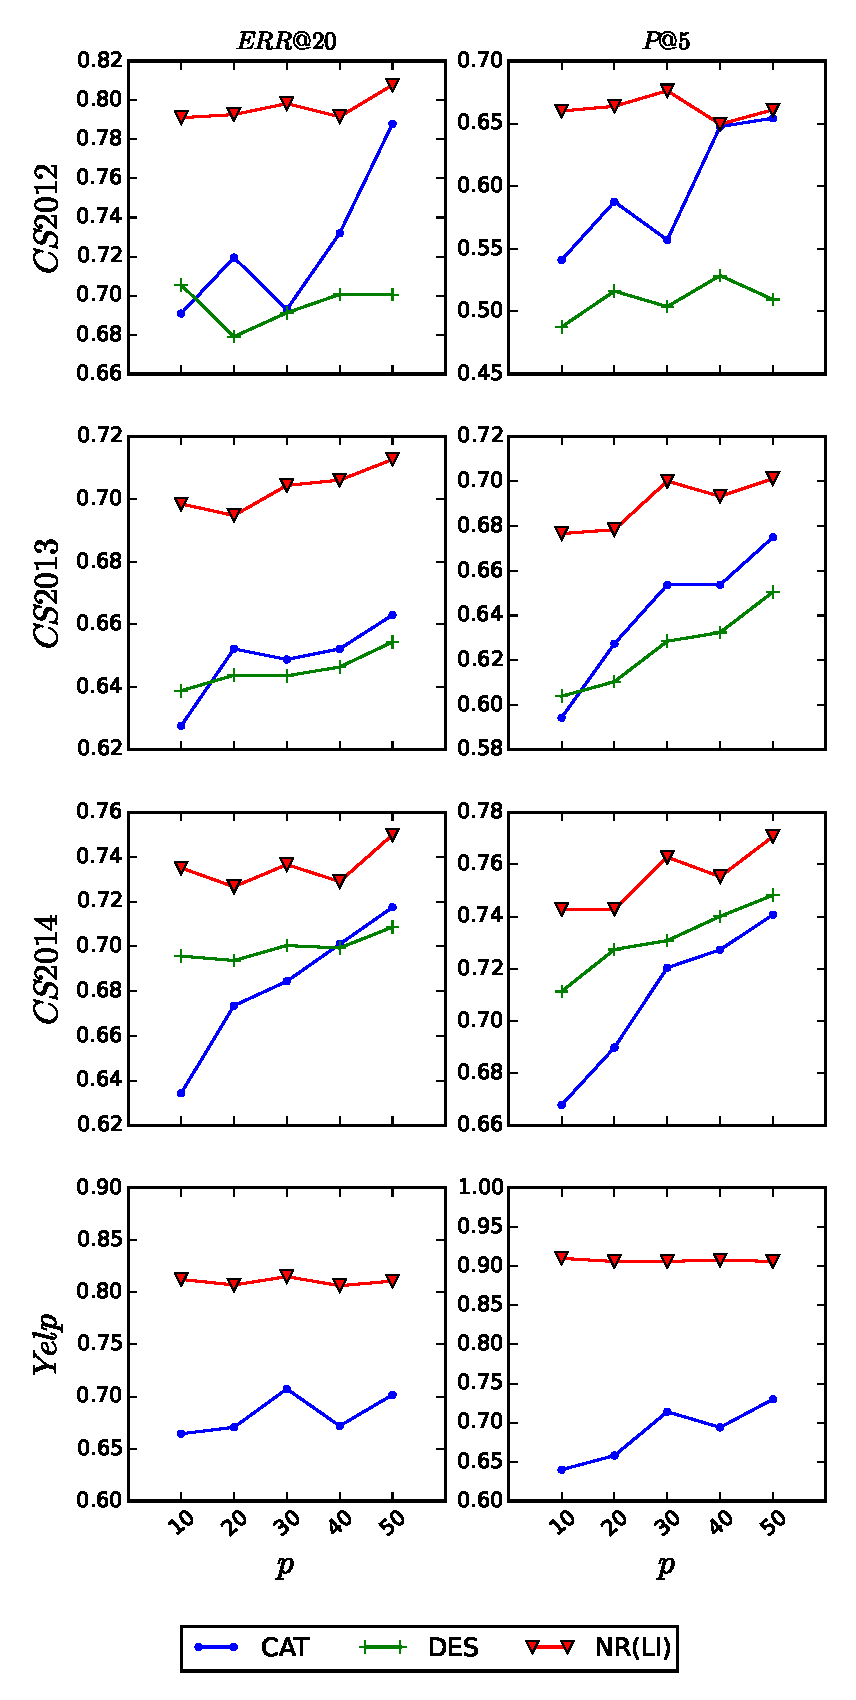
\includegraphics[scale=0.8]{figures/less-data-all.eps}
  \caption{The performance of using less data to build user profile}
  \label{fig:less_data_all}
\end{figure}




\begin{table}[t]
\centering
\caption{
Top frequent terms in different user profiles (id:918) and positive candidate profile (id:107)
}
\label{table:nr_analysis_top_up_terms}

\begin{tabular}{ |c|l|l| }
\hline
\multicolumn{3}{|c|}{\textbf{Positive User Profiles}} \\
\hline
\hline

NR & \multicolumn{2}{|l|}{\pbox{12cm}{place,burg,time,beer,food,chicago,wing,pie,art,chicken,kuma,\\view,bar,wait,day,drink,people,friend,table,hour,thing,cheese,\\sauce,night,fry}} \\ \hline
%& NEG & \pbox{10cm}{food,place,restaurant,time,wait,frontera,table,rick,hour,drink,\\bayless,service,reservation,bar,meal,thing,margarita,\\minute,grill,friend,experience,taco,appetizer,nothing,people} \\ \hline

FR & \multicolumn{2}{|l|}{\pbox{12cm}{burg,place,go,good,get,wait,time,great,beer,like,just,one,food,\\love,chicago,really,best,kuma,order,friend,will,also,\\back,bar,wing}} \\ \hline
%& NEG & \pbox{10cm}{food,wait,order,good,place,just,like,restaurant,mexico,time,\\get,frontera,bayless,table,rick,drink,hour,go,service,really,\\serve,want,eat,better,one} \\ \hline

SR & \multicolumn{2}{|l|}{\pbox{12cm}{order,go,burg,beer,worth,wing,will,went,well,way,want,wait,\\visit,view,two,try,time,though,think,take,table,sure,still,\\something,service}} \\ \hline
%& NEG & \pbox{10cm}{want,wait,thing,restaurant,order,hour,go,drink,worth,will,\\went,well,way,two,try,took,told,time,think,taco,table,\\small,since,service,serve} \\ \hline

RS & \multicolumn{2}{|l|}{\pbox{12cm}{great,good,place,best,burg,amaze,time,favorite,beer,pie,\\chicago,food,art,view,first,nice,ever,delicious,beautiful,fan,\\awesome,worth,wait,friend,free}} \\ \cline{2-3}
%& NEG & \pbox{10cm}{restaurant,good,food,mexico,service,mole,time,small,great,\\better,bayless,wait,place,fan,entree,year,worth,walk,sauce,rick,\\portion,minute,mediocre,long,huge} \\ \hline
\hline
\hline
\multicolumn{3}{|c|}{\textbf{Positive Candidate Profile}} \\ \hline
\textbf{Name} & \multicolumn{2}{|c|}{Little Goat} \\ \hline
\textbf{Description} & \multicolumn{2}{|l|}{\pbox{10cm}{Upscale diner next to the Little Goat Bakery serving \\breakfast items, sandwiches, burgers \& more}} \\ \hline

\multicolumn{3}{|l|}{\pbox{10cm}{goat,wait,little,good,food,great,order,place,like,dine,time,go,menu,love,just,\\try,back,friend,get,really,delicious,also,one,breakfast,sandwich,cheese,got,\\
table,pork,service,will,pancake,come,serve,coffee,well,can,amaze,definite,bread}} \\


\hline
\end{tabular}
\end{table}


\begin{table}[t]
\centering
\caption{
KL divergence between positive user profile (id:918) and positive candidate profile (id:107)
}
\label{table:nr_analysis_kl}

\begin{tabular}{ |c|c|c| }
\hline
Representations & KL Div. & Ranking \\
\hline
\hline
NR  & 1.54 & 7 \\ \hline
%& NEG & 1.63 &\\ \hline
FR  & 0.61 & 2 \\ \hline
%& NEG & 0.67 &\\ \hline
SR  & 1.40 & 2 \\ \hline
%& NEG & 1.41 &\\ \hline
RS  & 0.95 & 5 \\ \hline
%& NEG & 0.82 &\\ \hline
\end{tabular}
\end{table}


Previous results show that NR seems to be more robust and effective
than the other profile representations. Our result analysis suggests
that the better performance may be related to the fact that the 
NR-based profiles contain fewer noisy terms. Here, we use an example pair
i.e., user (uid:918) and candidate suggestion (id:107), to 
illustrate it. 
Table \ref{table:nr_analysis_top_up_terms} shows the most frequent
terms in the positive user profiles and the positive representation of
the candidate suggestion.
We can see that the candidate is about a place that selling
``breakfast items'' while the user seems to like ``beers'' and
``chicken wings''. Comparing these different profiles, it is
clear that the profiles generated by NR contain fewer noisy terms
than others.  When computing the similarity between the user
profile and candidate suggestions, these noisy terms could
mistakenly boost the ranking of the candidate suggestion.
This effect has been shown in Table \ref{table:nr_analysis_kl}.
We use KL-Divergence to measure the difference between
the user profile from the candidate representation.
It is clear that NR is able to capture difference between
the user profile and the candidate suggestion and rank
the suggestion at the seventh place.  On the other hand,
the other representations are more similar to the candidate
suggestion and incorrectly rank it at a higher place.

%\input{sec-exp_results_less_data}


\subsection{Experiments on Summary Generation}
\label{sec:results_summary}

We conduct two sets of experiments to evaluate the proposed structured
summary generation method. 

We first evaluate the quality of the summaries generated by the 
proposed method.  The baseline method is the snippet generation 
method developed by Yelp, and this method was used in one of the 
top ranked TREC runs \cite{adriel:overview2014}.  
To compare the results of the two methods, we develop an annotation 
interface as shown in Figure \ref{fig:comp_judge_scrnshot}. 
There are 2,109 unique suggestions from the TREC 2013 and 2014 
contextual suggesion tracks, and we generate the summary for 
each of them using the two methods.  For each suggestion, the annotation 
system would present the summary generated by the two methods, and 
annotators are expected to read the results and decide which one is 
better or choose ``Hard or Impossible to Decide''. Two annotators are hired 
for this task, and they are assigned to judge 1,300 and 1,209 
suggestions respectively. There are suggestions judged by both assessors 
so that we can see whether judgements between the two assessors 
are consistent. 

%The official judgements in TREC 2013 and 2014 Contextual Suggestion Task are based on pooling and only the top 5 results of each pooled (profile, context) pair are judged. The number of pooled (profile,context) pairs is 223 and 229 for TREC 2013 and TREC 2014 respectively. This results in 1115 and 1495 officially judged suggestions. After removing the duplicated suggestions there are 2109 unique suggestions left. We hire two graduate students from our department to annotate the better summary from our structured summary and baseline for each suggestion. The screen-shot of the web-based annotation system is shown in Figure \ref{fig:comp_judge_scrnshot}. Annotators are requested to figure out the better summary or choose ``Hard or Impossible to Decide'' if they cannot decide which one is better. Basically there is no hard criteria of the annotation. However, annotators achieve consensus on that better summary should provide more useful information as expected. We retain 400 (about 20\%) of the suggestions to test the agreement between the two annotators.

\begin{figure}[t]
  \centering
  
\includegraphics{figures/comp_judge_scrnshot.eps}
  \caption{Screen shot of the web-based annotation system to compare two summary generation methods}
  \label{fig:comp_judge_scrnshot}
\end{figure}


\begin{table}[t]
\centering
\caption{Comparison of results summarization methods}
\label{table:comp_summary_anno_results}
\begin{tabular}
{ |l|l|l| }
\hline
\multicolumn{3}{|l|}{\textbf{Overlapped Suggestions}} \\
%\hline
\hline
& Annotator\#1 & Annotator\#2 \\ \hline
Our method is better than the baseline. & 71\% & 86\% \\
Our method is worse than the baseline. & 20\% & 11\% \\
Hard or Impossible to decide & 9\% & 4\% \\
\hline
%\textbf{Agreement(Cohen's Kappa)} & \multicolumn{2}{|c|}{0.14} \\
%\hline
\hline
\multicolumn{3}{|l|}{\textbf{Non-Overlapped Suggestions}} \\
%\hline
\hline
& Annotator\#1 & Annotator\#2 \\ \hline
Our method is better than the baseline. & 78\% & 68\% \\
Our method is worse than the baseline. & 15\% & 32\% \\
Hard or Impossible to decide & 7\% & 0\% \\
%Annotator\#1 & \multicolumn{2}{|c|}{0.78} \\
%Annotator\#2 & \multicolumn{2}{|c|}{0.68} \\
\hline
\end{tabular}
\end{table}


The comparison results are shown in Table \ref{table:comp_summary_anno_results}. 
Among the overlapped suggestions, both annotators think that our method performs 
better than the baseline method for over 70\% of the suggestions. 
Similar observations can be made for the non-overlapped
suggestion set as well. Thus, it is clear that our structured summary 
generation method is more effective than the state of the art baseline 
method. 


Since each structured summary contains multiple components, we 
also conduct experiments to evaluate the effectiveness for each 
component. Note that the last component is personalized and it is 
trivial to evaluate its effectiveness, so we focus on evaluating
the first three components, i.e, opening, official introduction and 
review. We recruit three annotators (two of whom are the same
ones as in the previous task) to assess the quality of 
the structured summaries. Following the same judgement strategy 
used by TREC, there are 5 rating levels, and 0,1,2 are mapped 
to non-relevant and 3,4 are mapped to relevant.  
The interface of the annotation system is 
shown in Figure \ref{fig:summary_judge_scrnshot}. 
Again, there are 2,109 suggestions, and we split the job 
among three annotators. There are 200 suggestions assessed
by all the three assessors to measure the agreement. 
The results are evaluated with accuracy, i.e,. the number
of relevant summaries divided by the number of summaries. 

\begin{figure}[t]
  \centering
  
\includegraphics{figures/summary_judge_scrnshot.eps}
  \caption{Screen shot of the web-based annotation system to evaluate the effectiveness of components}
  \label{fig:summary_judge_scrnshot}
\end{figure}


Table \ref{table:summary_annotate_overlapped} shows the accuracy of 
each section for the overlapped suggestions. It is clear that all 
sections have high accuracy. Among them, it seems that the official 
introduction are less relevant than the other two components. 
We also measure the agreement among the three assessors, and the 
agreement is around 0.5 for the official introduction, 0.7 for 
the opening, and 0.6 for the review component. 
Furthermore, Table \ref{table:summary_annotate_all} shows the accuracy 
of each component for all suggestions including the ones shared 
among annotators. If a suggestion is from the overlapped set, i.e., 
having more than one annotation, the relevance status of a component 
is determined by the majority vote.  Since all the suggestions 
are from the pool of either TREC 2013 CS track or TREC 2014 CS track, 
we report the accuracy for each collection separately. 
The observation here is similar to what we observed in the overlapped set. 
It is clear that both opening and review components are useful and more 
relevant. 


\begin{table}[t]
\centering
\caption{Evaluation results on the overlapped suggestions (measured by accuracy)} 
\label{table:summary_annotate_overlapped}
\begin{tabular}
{ |l|c|c|c| }
\hline
Components & Annotator \#1 & Annotator \#2 & Annotator \#3 \\ \hline
%Whole & 0.69 & 0.81 & 0.92 \\ \hline
Opening & 0.98 & 0.81 & 0.80 \\ \hline
``Official'' Intro & 0.75 & 0.53 & 0.78 \\ \hline
Review & 0.87 & 0.95 & 0.99 \\ \hline

\hline

\end{tabular}
\end{table}

\begin{table}[t]
\centering
\caption{Evaluation results on all the suggestions (measured by accuracy)} 
\label{table:summary_annotate_all}
\begin{tabular}
{ |l|c|c| }
\hline
Components &   CS2013 & CS2014 \\\hline 
Opening & 0.99 & 0.83 \\ \hline
``Official'' Intro & 0.56 & 0.47 \\ \hline
Review & 0.69 & 0.77 \\ \hline

\hline

\end{tabular}
\end{table}



\section{Conclusions} 
\label{sec:con} 

%* Future work:   personalized local search \cite{Lv:12}. 
%* consider distance 
%* evaluate with TREC problem set up 

One of the important challenging in mobile search is
to return satisfying results based on not only 
user preference history but also contextual information. 
Our work focuses on user profiling for contextual suggestion. 
In particular, we propose to use opinions for both candidate 
suggestion ranking as well as suggestion summary generation. 

For candidate suggestion ranking task, category, description 
and opinions are used to build the enriched user profile and 
the candidate suggestion profile. 
For opinion based user profile several opinion representations 
including the full review text and part of the review text have 
been explored to model the user profile. 
Various ranking methods including linear interpolation and 
learning to rank have been investigated to compute the ranking scores. 
The effectiveness of our methods have been tested on standard TREC 
collections and a self-crawled Yelp collection for both P@5 and ERR@20. 
The more detailed analysis showed that using NR as the 
representation of the opinion in general performs better than other 
opinion representations. 
Although there is no obvious difference between the optimal performance 
of linear interpolation and learning to rank, MART performs better than 
other learning to rank methods - Lambda MART and Linear Regression.
We further did more in-depth analysis on how size of the user 
profile can affect the performance. The results showed that using as 
few as 10\% of the user preferences to build the user profile still 
leads to promising performance.

Furthermore, we also propose to construct a structured summary 
by leveraging information from multiple resources. Experiment results 
show that the proposed method is more effective than the baseline method, 
and some components in the summary are more useful than the others. 
